% Geometric interpretation of the ORCA planner -- step-by-step build for
% slides. One page per step (include in beamer via \includegraphics[page=N]):
%   1  workspace: robot A, pedestrian B, Minkowski radius r_A+r_B
%   2  velocity space: truncated VO translated by v_B; v_pref inside it
%   3  escape vector u + ORCA half-plane through v_A + (1/2)u
%   4  v_new = projection of v_pref onto the allowed half-plane
%   5  reciprocity: ghost VO shifted by -u/2 (B's half) is TANGENT to the
%      alpha=1/2 line -- why the line may cross the *current* VO
%   6  full yield alpha=1: line through v_A+u, tangent to the original VO
% Pages 2-6 share one bounding box, so overlaying them in a deck is stable.
% All coordinates are computed, not sketched: cone tangents for a disk of
% radius 1 at (3,1.2), tau=2, v_B=(-0.6,-0.2), v_A=(0.78,0.32),
% u=(-0.296,-0.198), n=(-0.832,-0.555).
% NOTE (matches orca.py, do not "fix"): with alpha=1/2 the projected v_new
% lies inside the *drawn* VO -- correct reciprocity, B simultaneously takes
% its half and the VO shifts. Only alpha=1 clears the VO unilaterally.
% Colors: dataviz palette, validated (blue A, orange B/VO, red u,
% green alpha=1/2, violet alpha=1).
% Compile: pdflatex orca_geometry.tex
\documentclass[tikz,border=10pt]{standalone}
\usepackage{amsmath,amssymb}
\usetikzlibrary{arrows.meta,calc}

\definecolor{cblue}{HTML}{2A78D6}
\definecolor{corange}{HTML}{EB6834}
\definecolor{cred}{HTML}{E34948}
\definecolor{cgreen}{HTML}{008300}
\definecolor{cviolet}{HTML}{4A3AA7}

\tikzset{
  every picture/.style={font=\sffamily\small, >={Stealth[length=2.2mm]}},
  vec/.style={->, very thick},
  lbl/.style={font=\sffamily\scriptsize, inner sep=1pt},
  steptitle/.style={font=\sffamily\small\bfseries, anchor=west},
  stepsub/.style={font=\sffamily\scriptsize, text=black!55, anchor=west},
}

% ---- shared velocity-space building blocks (pages 2-5) ----
\newcommand\velcanvas{%
  \useasboundingbox (-1.5,-1.75) rectangle (3.1,2.85);
  \draw[black!15] (-1.4,-1.6) rectangle (3.0,2.4);
  \draw[black!20, thin] (-1.4,0) -- (3.0,0);
  \draw[black!20, thin] (0,-1.6) -- (0,2.4);
  \fill[black] (0,0) circle (0.035);
  \node[lbl, anchor=north east] at (0,0) {$0$};}

\newcommand\allowedfill{%
  \begin{scope}\clip (-1.4,-1.6) rectangle (3.0,2.4);
    \fill[cgreen!8] (-2.14,4.38) -- (3.41,-3.94) -- (-3.25,-8.38)
                    -- (-8.8,-0.06) -- cycle;
  \end{scope}
  \node[lbl, cgreen!80!black] at (-0.75,-1.0) {allowed};}

\newcommand\stripfill{%
  \begin{scope}\clip (-1.4,-1.6) rectangle (3.0,2.4);
    \fill[black!6] (-2.14,4.38) -- (3.41,-3.94) -- (3.26,-4.04)
                   -- (-2.29,4.28) -- cycle;
  \end{scope}}

\newcommand\allowedfillone{%
  \begin{scope}\clip (-1.4,-1.6) rectangle (3.0,2.4);
    \fill[cviolet!8] (-2.29,4.28) -- (3.26,-4.04) -- (-3.40,-8.48)
                     -- (-8.95,-0.16) -- cycle;
  \end{scope}
  \node[lbl, cviolet, anchor=west] at (-1.3,-1.2) {allowed ($\alpha=1$)};}

\newcommand\ghostvo{%
  \begin{scope}\clip (-1.4,-1.6) rectangle (3.0,2.4);
    \begin{scope}[shift={(-0.452,-0.101)}]
      \draw[corange!80, densely dashed, thick]
        (1.5329,0.1010)
        arc[start angle=-86.2, end angle=-230.2, radius=0.5]
        -- (2.6877,2.2421)
        arc[start angle=39.83, end angle=3.77, radius=3.5]
        -- cycle;
    \end{scope}
  \end{scope}
  \fill[cgreen!80!black] (0.632,0.221) circle (0.035);
  \draw[black!45, ->, thin] (1.72,-0.52) -- (1.12,-0.05);
  \node[lbl, corange!60!black, anchor=west] at (1.62,-0.62)
       {VO after $B$'s half};}

\newcommand\projectionone{%
  \draw[black!50, densely dotted] (1.2,0.2) -- (0.668,-0.155);
  \draw[vec, cviolet, line width=1.4pt] (0,0) -- (0.668,-0.155);
  \node[lbl, cviolet, anchor=north east] at (0.62,-0.22) {$v_A^{\mathrm{new}}$};}

\newcommand\voshape{%
  \begin{scope}\clip (-1.4,-1.6) rectangle (3.0,2.4);
    \begin{scope}[shift={(-0.6,-0.2)}]
      \path[fill=corange!45, fill opacity=0.5, draw=corange, thick]
        (1.5329,0.1010)
        arc[start angle=-86.2, end angle=-230.2, radius=0.5]
        -- (2.6877,2.2421)
        arc[start angle=39.83, end angle=3.77, radius=3.5]
        -- cycle;
    \end{scope}
  \end{scope}
  \node[lbl, corange!60!black] at (1.80,1.42)
       {$\mathrm{VO}^{\tau}_{A|B} \oplus v_B$};}

\newcommand\orcaline{%
  \begin{scope}\clip (-1.4,-1.6) rectangle (3.0,2.4);
    \draw[cgreen, thick] (-0.589,2.051) -- (1.853,-1.609);
  \end{scope}
  \node[lbl, cgreen!80!black, anchor=south west] at (-0.62,2.09)
       {ORCA ($\alpha=\tfrac12$)};}

\newcommand\alphaoneline{%
  \begin{scope}\clip (-1.4,-1.6) rectangle (3.0,2.4);
    \draw[cviolet, thick, densely dashed] (-0.737,1.952) -- (1.705,-1.708);
  \end{scope}
  \node[lbl, cviolet, anchor=east] at (-0.80,1.86) {$\alpha=1$};}

\newcommand\uarrow{%
  \draw[vec, cred, line width=1.2pt] (0.78,0.32) -- (0.484,0.122);
  \node[lbl, cred, anchor=east] at (0.55,0.34) {$u$};}

\newcommand\vecbase{%
  \draw[vec, corange] (0,0) -- (-0.6,-0.2)
       node[lbl, corange!70!black, anchor=north east]{$v_B$};
  \draw[vec, cblue] (0,0) -- (0.78,0.32)
       node[lbl, cblue, anchor=south west]{$v_A$};
  \draw[vec, cblue, densely dashed] (0,0) -- (1.2,0.2)
       node[lbl, cblue, anchor=west]{$v_A^{\mathrm{pref}} \in \mathrm{VO}$};}

\newcommand\projection{%
  \draw[black!50, densely dotted] (1.2,0.2) -- (0.816,-0.056);
  \draw[vec, cblue, line width=1.4pt] (0,0) -- (0.816,-0.056);
  \node[lbl, cblue, anchor=north] at (0.70,-0.16) {$v_A^{\mathrm{new}}$};}

% heading intentionally omitted (slide frame provides it); subtitle only
\newcommand\steplabels[2]{%
  \node[stepsub] at (-1.4,2.6) {#2};}

\begin{document}

% ================= page 1: workspace =================
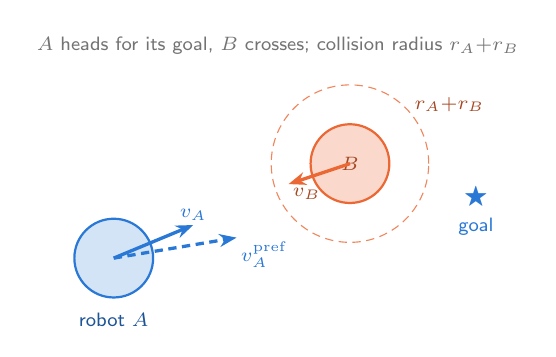
\begin{tikzpicture}
  \node[stepsub] at (-1.1,2.7)
       {$A$ heads for its goal, $B$ crosses; collision radius $r_A{+}r_B$};

  \fill[cblue!20] (0,0) circle (0.5);
  \draw[cblue, thick] (0,0) circle (0.5);
  \node[lbl, cblue!70!black] at (0,-0.78) {robot $A$};

  \fill[corange!25] (3,1.2) circle (0.5);
  \draw[corange, thick] (3,1.2) circle (0.5);
  \node[lbl, corange!70!black] at (3,1.2) {$B$};
  \draw[corange!80, densely dashed] (3,1.2) circle (1.0);
  \node[lbl, corange!70!black, anchor=west] at (3.78,1.95) {$r_A{+}r_B$};

  \draw[vec, corange] (3,1.2) -- (2.22,0.94)
       node[lbl, corange!70!black, anchor=north west]{$v_B$};
  \draw[vec, cblue] (0,0) -- (1.01,0.42)
       node[lbl, cblue, anchor=south]{$v_A$};
  \draw[vec, cblue, densely dashed] (0,0) -- (1.56,0.26)
       node[lbl, cblue, anchor=north west]{$v_A^{\mathrm{pref}}$};
  \node[cblue, font=\small] at (4.6,0.77) {$\bigstar$};
  \node[lbl, cblue, anchor=north] at (4.6,0.55) {goal};
\end{tikzpicture}

% ================= page 2: the velocity obstacle =================
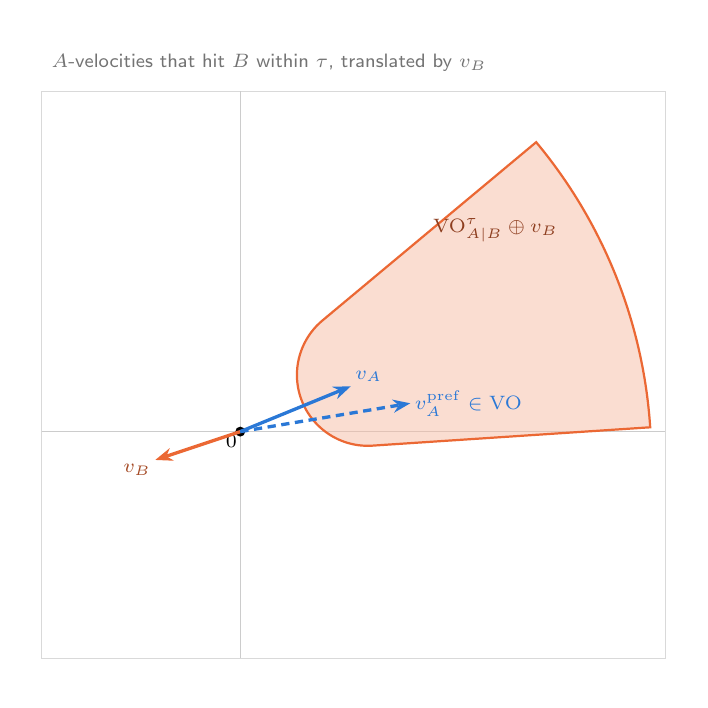
\begin{tikzpicture}[scale=1.8]
  \steplabels{Step 2 -- The velocity obstacle}
             {$A$-velocities that hit $B$ within $\tau$, translated by $v_B$}
  \velcanvas
  \voshape
  \vecbase
\end{tikzpicture}

% ================= page 3: one linear constraint =================
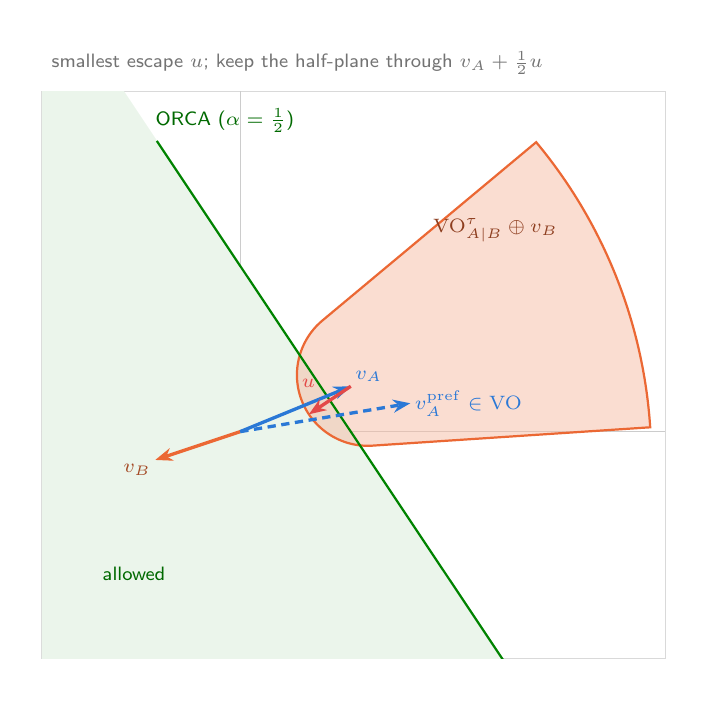
\begin{tikzpicture}[scale=1.8]
  \steplabels{Step 3 -- One linear constraint}
             {smallest escape $u$; keep the half-plane through $v_A + \tfrac12 u$}
  \velcanvas
  \allowedfill
  \voshape
  \orcaline
  \vecbase
  \uarrow
\end{tikzpicture}

% ================= page 4: the new velocity =================
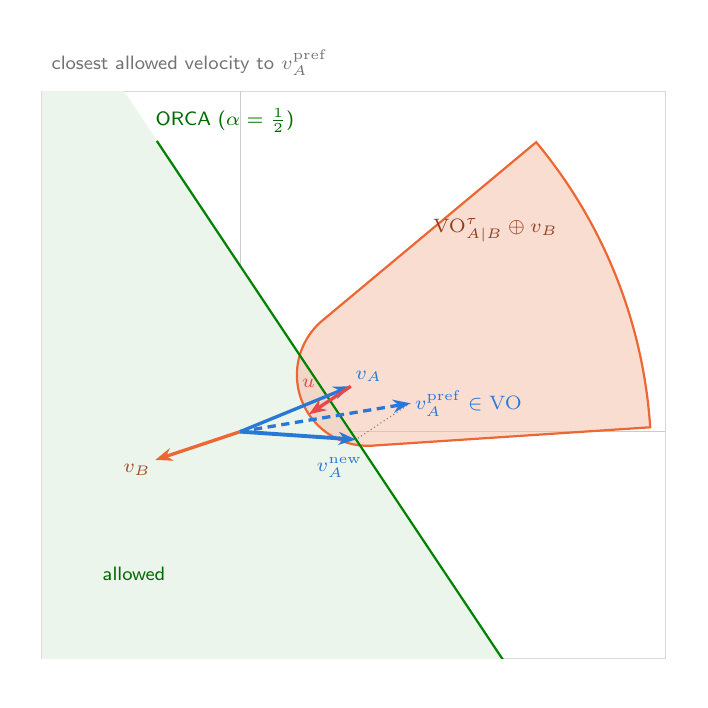
\begin{tikzpicture}[scale=1.8]
  \steplabels{Step 4 -- The new velocity}
             {closest allowed velocity to $v_A^{\mathrm{pref}}$}
  \velcanvas
  \allowedfill
  \voshape
  \orcaline
  \vecbase
  \uarrow
  \projection
\end{tikzpicture}

% ================= page 5: reciprocity =================
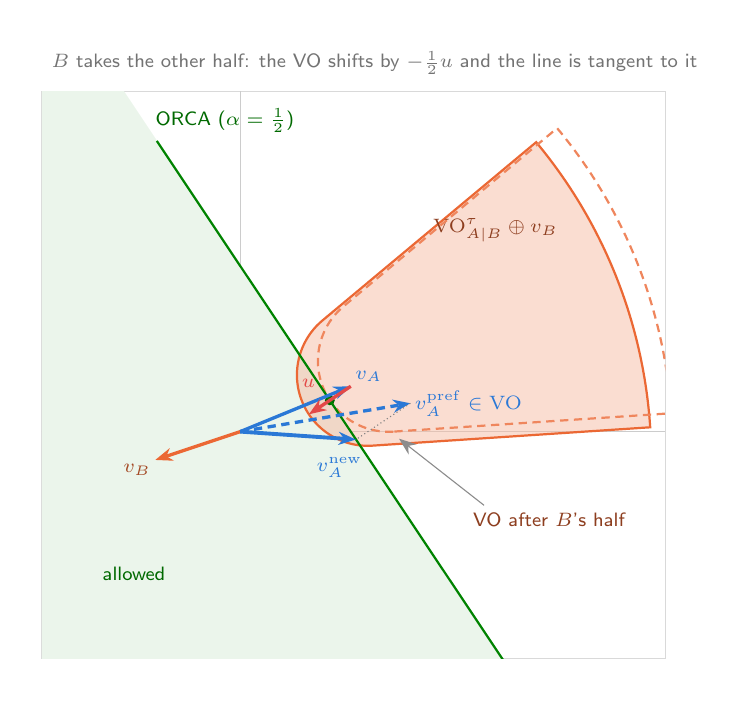
\begin{tikzpicture}[scale=1.8]
  \steplabels{Step 5 -- Reciprocity: crossing the VO is fine}
             {$B$ takes the other half: the VO shifts by $-\tfrac12 u$ and the line is tangent to it}
  \velcanvas
  \allowedfill
  \voshape
  \ghostvo
  \orcaline
  \vecbase
  \uarrow
  \projection
\end{tikzpicture}

% ================= page 6: full yield =================
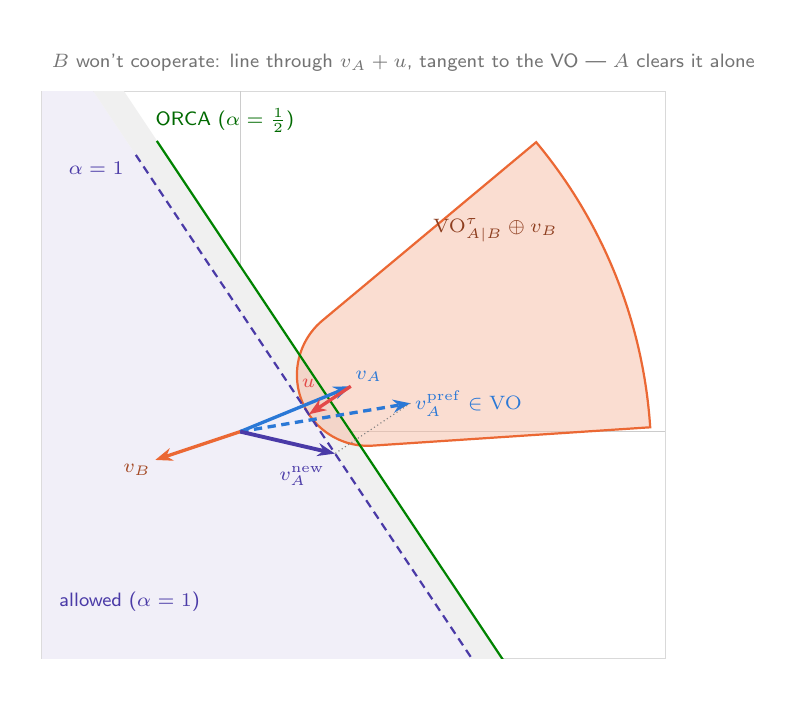
\begin{tikzpicture}[scale=1.8]
  \steplabels{Step 6 -- Full yield ($\alpha=1$)}
             {$B$ won't cooperate: line through $v_A + u$, tangent to the VO --- $A$ clears it alone}
  \velcanvas
  \allowedfillone
  \stripfill
  \voshape
  \orcaline
  \alphaoneline
  \vecbase
  \uarrow
  \projectionone
\end{tikzpicture}

\end{document}
